%1. ¿La entropía de la fuente S es máxima? ¿Que sugiere esto acerca de la red? ¿Está relacionado con el
%overhead impuesto por la red debido a los protocolos de control (i.e.: ARP)?
\textbf{Datos obtenidos con la fuente $S$:}

\begin{center}
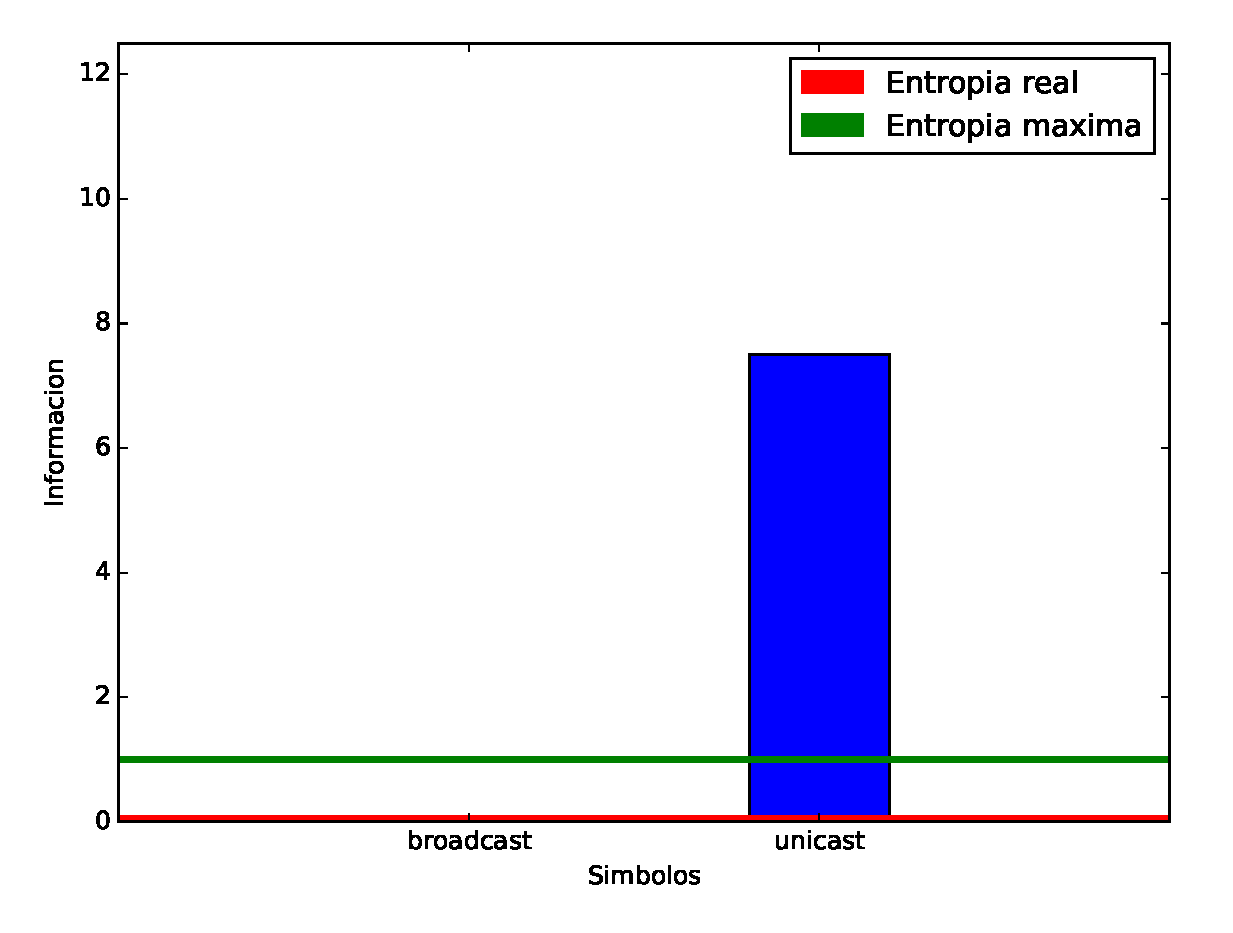
\includegraphics[scale=0.6]{imagenes/analisisTCORPcableada/fuenteS.eps} 
\end{center}

Como se puede observar hay muchísimos más broadcast que unicast, es por ello que el último dá más información. Las probabilidades son las siguientes: broadcast 0.99, unicast 0.01. La entropía es 0.049, casi nula.\\

Los broadcast son visibles para todos los dispositivos, mientras que los unicast no. Al ser una red grande, nosotros estamos viendo los broadcast de todos los hosts y sólo nuestros unicast (respuestas enviadas al host con el cuál se hizo la captura), es por esto que la diferencia es tan grande.\\

%2. ¿Cómo es el tráfico ARP en la red? ¿Se pueden distinguir nodos? ¿Cuántos? ¿Indica algo la cantidad?
%¿Se les puede adjudicar alguna función específica? ¿Hay evidencia parcial que sugiera que algún nodo
%funciona de forma anómala y/o no esperada?
%3. ¿Existe una correspondencia entre lo que se conoce de la red y los nodos distinguidos detectados por
%la herramienta? ¿Es posible usar el criterio de distinción propuesto como método para descubrir el/los
%Default Gateway/s de la red? ¿Es preciso?
\textbf{Datos obtenidos con la fuente $S1$:}

\begin{center}
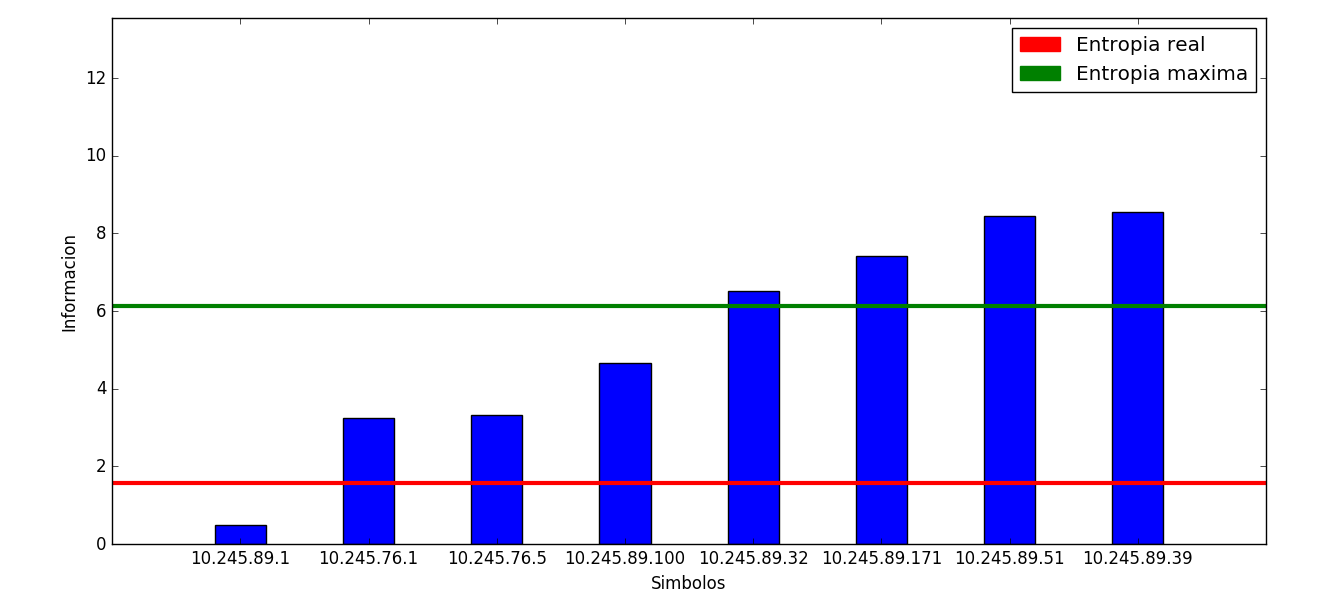
\includegraphics[scale=0.45]{imagenes/analisisTCORPcableada/fuenteS1.png} 
\end{center}




